\chapter{Simulator}
\label{chapter:simulator}

Testing and evaluating a peer-to-peer protocol with thousands of nodes in a real environment is very difficult, expensive and time consuming, especially if the goal is to evaluate the effects of large-scale network attacks.
For this reason, we decided to implement a simulator that measures the performances of the Bitcoin protocol under the different situations, at rest and under attack.
This allowed us to simulate up to \num{10000} Bitcoin nodes on a single general-purpose computer in a short time and evaluate the behavior of the protocol under different attack scenarios.

\medskip
This chapter describes the implementation of the simulator.
It covers the main concepts of discrete event simulation, the basics of PeerSim, the design of the simulator, the simplifications with respect to the complete Bitcoin protocol, and the metrics used to measure and evaluate the overall performances.


\section{Simulation}
According to Robert E. Shannon, \textit{simulation} is ``the process of designing a model of a real system and conducting experiments with this model for the purpose of understanding the behavior of the system and / or evaluating various strategies for the operation of the system'' \cite{simulation_shannon_1998}.
By \textit{model}, he means an abstract representation of an entity of group of objects, and by \textit{system} a collection of elements that interact with each other to accomplish some objective.
According to Shannon, simulation has a number of advantages \cite{simulation_shannon_1998}:
\begin{itemize}
	\item it is often easier to understand than analytical or mathematical models;
	\item it is usually more credible than models, since it requires less simplifying assumptions and represents the system more accurately;
	\item it allows to test new designs, systems or protocols before implementing them;
	\item it allows to verify hypothesis by measuring their effects on the systems;
	\item it helps to understand better how the modeled system works and which variables are the most important with respect to the performances;
	\item it allows to changes the initial situation and test the system in different settings.
\end{itemize}

\medskip
Simulation is used in many contexts, for example safety engineering, economics, physics and even video games \cite{wikipedia_simulation}.
There are many different approaches to simulations, each one adapted to a specific purpose.
We focus on discrete event simulation, used by our simulator.


\section{Discrete event simulation}
A discrete event simulation models the system behavior as a discrete sequence of events in time.
An event can represent anything, for example the arrival of a message to a node in the system or a network timeout.
Each event occurs at a particular instant of time and can cause changes in the state of the system.
No event occurs between \num{2} consecutive events, so the simulation can simply jump from one event to the next.
The results of the simulation can be evaluated with measurements:
the metrics can be computed either online during the simulation run, or computed offline from the simulation logs.

\medskip
\begin{algorithm}[h]
	\setstretch{1.15}
	\DontPrintSemicolon

	\SetKw{New}{new}
	\SetKwData{State}{state}
	\SetKwData{Events}{events}
	\SetKwData{Queue}{queue}
	\SetKwData{Event}{event}
	\SetKwData{NewState}{newState}
	\SetKwData{NewEvents}{newEvents}
	\SetKwFunction{InitializeState}{initializeState}
	\SetKwFunction{InitializeEvents}{initializeEvents}
	\SetKwFunction{PriorityQueue}{PriorityQueue}
	\SetKwFunction{IsEmpty}{isEmpty}
	\SetKwFunction{DeleteMin}{deleteMin}
	\SetKwFunction{InsertAll}{insertAll}
	\SetKwFunction{ProcessEvent}{processEvent}
	\SetKwFunction{ExitConditionReached}{exitConditionReached}

	\BlankLine
	\CommentSty{// initialization} \;
	\State $\leftarrow$ \InitializeState{} \;
	\Events $\leftarrow$ \InitializeEvents{} \;
	\Queue $\leftarrow$ \New \PriorityQueue{\Events} \;

	\BlankLine
	\BlankLine
	\CommentSty{// simulation loop} \;
	\While{$\neg$ \Queue.\IsEmpty{} or \ExitConditionReached{\State}}{

		\BlankLine
		\CommentSty{// process the next event} \;
		\Event $\leftarrow$ \Queue.\DeleteMin{} \;
		\NewState, \NewEvents $\leftarrow$ \ProcessEvent{\Event} \;

		\BlankLine
		\BlankLine
		\CommentSty{// update the system status} \;
		\State $\leftarrow$ \NewState \;
		\Queue.\InsertAll{\NewEvents} \;

		\BlankLine
	}
	\BlankLine

	\caption{Discrete Event Simulator}
	\label{alg:des}
\end{algorithm}
\smallskip

\cref{alg:des} illustrates the working of a discrete event simulation engine.
The simulation has some starting state that represents the initial condition of the system.
All events are stored in a priority queue sorted by event time.
The queue is initialized with some events.
Events in the queue are processed one at a time:
the first event is removed from the queue and processed by the simulator.
An event can cause other events to occur in the future and change the current state if the system.
Discrete event simulators take advantage of pseudorandom number generators to emulate random variables of the system \cite{wikipedia_des}:
whenever an event is influenced by some random factor external to the system (e.g. latency of a TCP connection over the Internet), the simulator extracts a random variable from some distribution using the random number generators.
The simulation stops when a certain condition is reached (for example, a target simulation time is reached), or when the queue of events is empty.


\section{PeerSim}
PeerSim \cite{peersim_2009} is an open source peer-to-peer systems simulator engine developed at the University of Bologna and the University of Trento.
It is written in Java and aim is to help the research and evaluation of large peer-to-peer.
It has been developed with high scalability in mind, in order to support simulations with up to \num{1} million nodes.
It is released under the GPL open source license and is available for download on SourceForce \cite{peersim_site}.

\medskip
PeerSim is composed of two simulation engines, a simplified cycle-based one and an event-driven one.
The cycle-based engine uses some simplifying assumptions to achieve better performances and scalability, such as ignoring the details of the transport layer in the communication protocol stack;
it has been tested up to \num{1} million nodes \cite{peersim_intro_2018}.
The event-based engine is less efficient but more realistic and allows to easily simulate the entire network stack;
it has been used for simulation of up to \num{250000} nodes \cite{peersim_intro_2018}.
Both engines support many simple and extendable components, which are plugged together through a flexible configuration mechanism.
Since our simulator is event driven, this chapter focuses on the event-based engine only.

\subsection{Components}
Each component in PeerSim is created as a simple Java object that implements some interfaces defined by the engine.
\cref{fig:peersim} gives an overview of the main components of a PeerSim simulation.

\begin{figure}[ht]
	\centering
	\vspace*{0.25cm}
	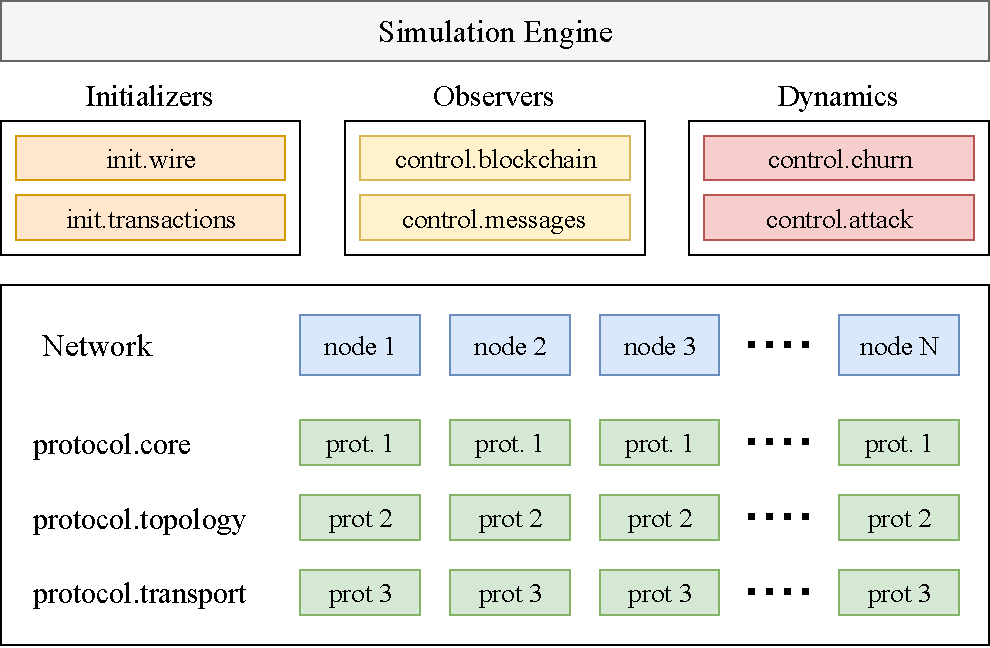
\includegraphics[scale=0.9]{figures/peersim}
	\vspace*{0.2cm}
	\caption[Illustration of the main components of PeerSim]{Illustration of the main components of PeerSim.}
	\label{fig:peersim}
\end{figure}

\subsubsection{EDSimulator}
The \texttt{EDSimulator} is a static singleton that implements the event-driven simulator engine.
It is the entry point of each simulation and it is responsible to manage its entire life-cycle:
load the configuration, bootstrap the network, run the initializers, keep the queue of events, schedule controls, and run the simulation loop.
It provides a method that can be used by any component to add new events to the queue.
The class is also able to run the same simulation multiple times using different seeds for the random number generators, in order to achieve a higher statistical significance.

\subsubsection{Event}
PeerSim does not have any class or interface to model an event.
Events are simply represented as plain Java objects, which are passed by reference to the simulator engine and to the target components.

\subsubsection{Network}
The \texttt{Network} class is a static singleton that keeps track of all nodes in the simulation.
Nodes are internally stored in an array and can be accessed by ID (their position in the array).
Information about neighbors of a node is stored in a special protocol \texttt{Linkable}.
It is used by all components that need to access a specific node or iterate over the available nodes.

\subsubsection{Node}
The network is composed of nodes.
A node is a container of protocols (each simulation can have \num{1} or more protocols).
The \texttt{Node} interface provides access to the protocols it holds, and to a fixed unique identifier of the node.
The behavior of a node is defined in each of the attached protocols.

\subsubsection{EDProtocol}
The \texttt{EDProtocol} interface defines a protocol that implements an event-driven behavior.
Protocols define the actions each node will perform during the simulation.
The interface has only the method \texttt{processEvent}, which is invoked by the scheduler to deliver events to the protocol.
Each node stores an array or protocols;
a class implementing this interface will have \num{1} instance for each node in the network.
Protocols can be stacked on each other to build more and more complex behaviors:
for example, an implementation of \texttt{EDProtocol} might be responsible to build and maintain a topology, while a second implementation may simulate some higher level functions, such as broadcasting some objects to the entire network in a gossip style using the underlying topology.
The simulation settings are specified with a configuration file;
some settings can be overridden with command line parameters.

\subsubsection{Linkable}
The \texttt{Linkable} interface provides a service to other protocols to access a set of neighbor nodes.
The instances of the same linkable class define an overlay network:
each instance has a list neighbors nodes.
Links do not need to be symmetric:
in some cases it could make sense to work with a directed graph.
The \texttt{Linkable} interface is usually implemented by protocols that exchanges messages over the network to build a topology.

\subsubsection{Transport}
The \texttt{Transport} interface models a transport layer in the OSI model \cite{wikipedia_osi}:
it is used to send messages through the underlying network.
Implementations of the \texttt{Transport} interface use the \texttt{EDSimulator} class to schedule the delivery of messages with some appropriate delay.
They can also model packet loss of packets and other failures.
Different transports can be stack on top of each other to model complex behaviors of the network.

\subsubsection{Control}
Classes implementing \texttt{Control} are used to define operations that require global network knowledge and management.
They can be scheduled for execution at certain points during the simulation, depending on their function.

\paragraph{Initializers}
Initializers are executed at the beginning of the simulation and are used to bootstrap the simulation.
Examples include creating the initial network topology, set the initial nodes' states and schedule the first events.

\paragraph{Dynamics}
Dynamics are executed periodically during the simulation and are used to modify the simulation in some way.
Examples include adding or removing nodes, creating a failure on the network, and introducing an extra delay for messages.

\paragraph{Observers}
Similar to dynamics, observers are executed periodically during the simulation.
They are used to read aggregated valued from nodes, and compute and collect statistics and metrics.

\subsubsection{Configuration}
\texttt{Configuration} is a static singleton class that provides access to the configuration for the current simulation.
It proxies all accesses to the configuration file and it allows to plug different strategies to load the configuration.
The configuration is stored as \texttt{<name, value>} pairs.
The class provides helper methods to perform common operations, such as reading values with type checking, resolving protocols by name, parsing mathematical expressions (that can be used in the configuration file), and resolving under-specified class-names.

\subsubsection{CommonState}
\texttt{CommonState} is a singleton static class that stores the state common to all components in the simulation.
Its main purposes is to simplify the simulator structure and increase the efficiency by avoiding some parameters passing.
It provides access to an instance of a pseudorandom number generator, already initialized with the provided seed and ready for use:
all components should use this instance to guarantee reproducibility of results.
Also, it stores the current time of the simulation.

\subsubsection{RangeSimulator}
The \texttt{RangeSimulator} is a utility class able to run simulations with ranges of parameters specified in the configuration file.
A range is a collection of values to be assigned to a variable.
If multiple ranges are specified, the class runs a simulation for all the possible combinations of values.
\texttt{RangeSimulator} invokes the standard PeerSim simulator engine to run each single experiment.

\subsection{Simulation life cycle}
Each PeerSim simulation has the following life cycle:
\begin{itemize}
	\item load and validate the configuration; the configuration file defines which components are used and how they interact;
	\item run the initializers, in the order provided in the configuration file;
	\item schedule dynamics and observers, according to the parameters specified in the configuration;
	\item start the simulation loop and process one event at a time, until the maximum simulation time is reached, the queue of events is empty or some control terminates the simulation;
	\item run the controls scheduled for execution after the simulation;
	\item cleanup and schedule the next repetition of the experiment.
\end{itemize}


\section{Simulator design}
Our simulator implements the Bitcoin protocol.
Since the final aim is to evaluate the effect of large scale network attacks against the protocol, we put particular emphasis on the details of the topology layer described in \cref{sec:topology};
the core layer (\cref{sec:core}) is a bit simplified and does not cover the advanced features of Bitcoin transactions.

\smallskip
The code is divided into \num{4} main parts: topology, core, optimized data structures and utilities, and attack.
Topology and core have their own Java packages, which contain events, messages, initializers, and observers specific to the PeerSim protocol.

\subsection{Topology}
The topology layer is implemented as a \texttt{EDProtocol} that implements the \texttt{Linkable} interface:
it is responsible to build the overlay network that the core layer uses to propagate blocks and transactions.
Its main functions are to bootstrap the network (when a new node join, it needs to discover some peer and connect to them) and to maintain the topology.

\medskip
\noindent
The discovery mechanism is simulated as follows:
\begin{itemize}
	\item nodes start with empty lists of incoming and outgoing connections;
	\item an initializer simulates the DNS peer discovery mechanism by populating the list of known peers of each node with about \num{25} randomly selected nodes;
	\item an initializer schedules a special event \texttt{StartEvent} to each node;
	\item nodes start the protocol and begin to connect to some known nodes, in order to open up to \num{8} outgoing connections;
	\item when a connection is established, nodes exchange \texttt{Addr} messages; at the same time, nodes start to exchange \texttt{Ping} and \texttt{Pong} messages to maintain the newly build topology;
	\item nodes propagate the \texttt{Addr} messages, as described in \cref{sub:address-propagation}.
\end{itemize}
The backup discovery mechanisms based on hard-coded seeds, database of known addresses and daemon configuration are not implemented.
Our implementation covers the behavior of the protocol under normal conditions.

\subsubsection{Simplifications}
The implementation of the topology layer covers almost all details explained in \cref{chapter:protocol}.
In order to make the simulation faster to run and easier to understand, we simplified some details of the protocol:
\begin{itemize}
	\item all nodes have a single IP address and are reachable from each other node;
	\item all nodes follow the protocol, so there is no need to maintain a ban list or to implement the \texttt{Reject} control message;
	\item all nodes are miners and run exactly the same version of the protocol, so the \texttt{Version} and \texttt{VerAck} messages are simplified;
	\item nodes do not crash or leave the network; since we simulate large scale attacks over small periods of time, we do not expect a significant churn in nodes in the network.
\end{itemize}

\subsubsection{Metrics}
Each node in the simulator records a number of metrics, which are periodically collected and aggregated by the observers:
\begin{itemize}
	\item number of messages sent to other peers, grouped by type;
	\item number of nodes removed because of timeouts;
	\item overall distribution of the number of connections established by each node.
\end{itemize}
The metrics are mainly to used check if the behavior of the topology layer is reasonable and thus to verify that the implementation is correct.

\subsection{Core}
The core layer is implemented as another \texttt{EDProtocol}, which uses the topology layer as a \texttt{Linkable} implementation.
The main functions are to simulate discovery and propagation of blocks and gossip of transactions.

\paragraph{Transactions}
Transactions are scheduled by an initializer.
Before the simulation, the initializer generates a list of transactions according to a Poisson process \cite{wikipedia_poisson_process}:
each transaction is scheduled to a single node, chosen following a uniform probability distribution.
During the simulation, each transaction is received as an event by a single node, which then sends it to its neighbors.
Eventually, all nodes in the network receive the transaction.

\paragraph{Blocks}
Each block contains a series of transactions and must include the solution to computational puzzle to be valid.
We assume that all nodes in the network mine blocks independently from each other (we do not model mining pools) and have the same computational power.
To solve the challenge, each node uses a brute-force approach and tries difference nonces, until a valid value is found or another node completes the current block.
We observe that:
\begin{itemize}
	\item the probability of success in a single nonce trial is negligible (Bitcoin regulates the target so that one block is published every \num{10} minutes on average);
	\item each miner solves a different problem, since its address is included in the block;
	\item peers compute the \ac{PoW} independently; as such, the probability that one of them succeeds does not depend on the progress of the other nodes;
	\item the time spent on the previous block does not influence the time needed to find the next one;
	\item miners stop the search and start from scratch with a new block frequently.
\end{itemize}
For these reasons, we model each single miner as a Poisson process:
the time expected for a single miner to complete a block follows an exponential distribution.

\medskip
To simulate the mining process, each node $x$ extracts a random variable $\delta$ from an exponential distribution and schedules the discovery of the next block at time $t + \delta$, where $t$ is the current simulation time.
If another node $y$ publishes a block in the time interval $[t, t + \delta]$, the node $x$ stop the process and schedules the next block from instant it receives the block from $y$;
the block scheduled for time $t + \delta$ is cancelled.
As soon as a node manages to finish a block, it broadcast it to all the neighbors and schedules the next one.

\subsubsection{Simplifications}
Since the focus of the simulation is to evaluate the performances of the protocol under different network conditions, we have a series of simplifications:
\begin{itemize}
	\item transactions are represented as simple tuples \texttt{\textlangle sender, amount, receiver\textrangle}, instead as a sequence of instructions written in a custom scripting language;
	\item since all nodes join the network together, there is no need to implement the initial block download procedure;
	\item all nodes behave correctly, so there is no need to verify the signature of transactions or the proof-of-work of blocks;
	\item all nodes in the network perform some mining;
	\item all miners have the same computational power.
\end{itemize}

\subsubsection{Metrics}
The main metric used to measure the performances of the core layer is the number of forks in the blockchain:
a fork is a branch of the chain different from the longest chain.
The simulator knows the global state of the simulation:
it is easy to compute the longest chain, observe forks and their lengths in a any given moment.
The metric considers all blocks known to the simulator, even if they have been just discovered and not yet known to all peers in the network.

\subsection{Data structures and utilities}
The simulator uses custom data structures optimized for some specific tasks.
Other utilities include a class to run range simulations in parallel and the implementation of the exponential probability distribution.

\subsubsection{CircularQueue}
\texttt{CircularQueue} is an implementation of a queue based on an array.
It allows to add elements to the queue, read or remove the oldest element, check if the queue is empty.
The elements are stored in the array, starting from left to right;
new elements are always added to the right size, old elements are removed from left.
\num{2} pointers keep track of the first and last element in the array.
The queue is able to automatically resize in the underlying array is full:
when a new element is added and the queue in full, an array with double capacity is allocated and all elements are moved there.
The cost of the enqueue operation in this scenario is $\mathcal{O}(n)$, where $n$ is the original capacity of the queue;
since the operation is performed only once every $n$ inserts, the amortized cost of the operation is $\mathcal{O}(1)$.
All other operations have always $\mathcal{O}(1)$ cost, since elements are stored in an array.

\medskip
\begin{algorithm}[h]
	\setstretch{1.15}
	\DontPrintSemicolon

	\SetKw{New}{new}
	\SetKw{Void}{void}
	\SetKw{Boolean}{boolean}
	\SetKw{Integer}{integer}
	\SetKw{Object}{object}

	\SetKwFunction{CircularQueue}{CircularQueue}
	\SetKwFunction{Enqueue}{enqueue}
	\SetKwFunction{Dequeue}{dequeue}
	\SetKwFunction{Head}{head}
	\SetKwFunction{IsEmpty}{isEmpty}

	\BlankLine
	\CommentSty{// constructor} \;
	\textsc{CircularQueue} \CircularQueue{\Integer n} \;

	\BlankLine
	\CommentSty{// add an element to the queue} \;
	\Void \Enqueue{\Object item} \;

	\BlankLine
	\CommentSty{// remove the oldest element from the queue} \;
	\Object \Dequeue{} \;

	\BlankLine
	\CommentSty{// get without removing the oldest element from the queue} \;
	\Object \Head{} \;

	\BlankLine
	\CommentSty{// check if the queue is empty} \;
	\Boolean \IsEmpty{} \;

	\caption{CircularQueue}
	\label{alg:circular-queue}
\end{algorithm}
\smallskip

The \texttt{CircularQueue} data structure is used in the implementation of the topology layer to handle the \texttt{Addr} messages propagation:
\texttt{Addr} messages are usually not immediately sent to the target node:
at each round, a random peer is selected and its queue of \texttt{Addr} messages is flushed (see the trickling procedure described in \cref{sub:address-propagation}).
The queue for each peer is potentially unbounded, so the implementation needs to be dynamically resized when needed.
The common operations are enqueue (to schedule a new \texttt{Addr} message) and dequeue (to flush the queue):
all operations have $\mathcal{O}(1)$ cost.

\subsubsection{ParallelSimulator}
The \texttt{ParallelSimulator} is a utility class able to handle ranges and generate the list of their combinations:
parameters are read from the configuration file using the standard PeerSim mechanisms;
the class computes their combination and prints them as a list of commands, ready to be executed from the command line.
This class is particular useful when combined with the GNU Parallel, a shell tool for executing jobs in parallel using one or more computers \cite{gnu_parallel}.
Discrete event driven simulations are very difficult to parallelize, since events have causal relationships which are usually not well known in advance and are influenced by random variables:
in other words, they run on a single core do not exploit modern multi-core \ac{CPU}s.
If the memory footprint is not the bottleneck, is is possible to reduce the total completion time of a simulation with range parameters by running them in parallel, one per available core:
\texttt{ParallelSimulator} generates the list of jobs to execute, which are then run by GNU Parallel in parallel.

\subsection{Attack}
The attack simulates a Balance attack, described in \cref{sec:balance}.
The balance attack was originally tested against Ethereum, but it is thought to work also against Bitcoin.
The attacker tries to partition the nodes into \num{2} groups with the same computational power:
nodes do not see the blockchain status of the other group and are likely to mine conflicting blocks.
In other works, the network generates many forks that the attacker can exploit to perform double-spending attacks, as detailed in \cref{sec:double-spending}.

\bigskip
The implementation of the Balance attack in PeerSim is based on a custom \texttt{Transport} class named \texttt{BalanceAttackTransport}:
the class partition the nodes based on their IDs in \num{2} groups and delays the propagation of \texttt{Block} messages between different groups.
The custom transport is stacked on top of the other transport layers used in the normal simulation.
There is no need to modify any other component of PeerSim:
the attack can be activated or deactivated using the standard configuration mechanism.
The same mechanism is used to specify the ``intensity'' of the attack in terms of \textit{delay} applied to \texttt{Block} messages.
Finally, it is possible to specify a \textit{delay} drop probability.
Please note that the original paper \cite{balance_attack_2017} does not talk about dropping messages;
however, since the attacker has control of the network, it is able to selectively delay of drop any message between pair of nodes.
We evaluate the effect of both factors in \cref{chapter:results}.
